\documentclass[../Main.tex]{subfiles}

\begin{document}

\section{Introduction}

Geometric Numerical Integration, when considered on the grand timeline of Mathematics, is a field still in its younger days. While work on the numerical treatment of differential equations had started off towards the end of the 19\textsuperscript{th} Century, it wasn't till the 1980s that numerical analysts shifted their focus onto Geometric Numerical Integration.  A  better part of the century had been involved in improving quantity -  producting methods that could produce accurate results without being computationally strenuous. But the interest in running computer simulations over longer time intervals revealed that quality was equally important. Most methods could accurately reflect properties of a system, such as its asymptotic time behaviour or its sensitivity to changes in initial conditions; not all could preserve attributes such as total enery or momentum - properties that are invariants to the flow of the differential equation.

Consider, for example \cite{Hairer2006}, the following set of Lotka-Volterra prey-predator equations:
\begin{align}
	\frac{du}{dt} = u - uv, \qquad \frac{dv}{dt} = uv - 2v \label{lotka-volterra_example}
\end{align} where $u(t)$ is the population of the prey over time, and $v(t)$ is that of the predator. Dividing the two equations in \ref{lotka-volterra_example}, we get that
\begin{align*}
\left(1 -  \frac{2}{u}\right) du = \left(\frac{1}{v} - 1\right) dv
\end{align*}
Integrating the two sides of the equation, we get that
\begin{align}
I(u, v) = u - 2\ln{u} +  v - \ln{v} = const \label{lotka-volterra_solution}
\end{align}
giving us that the solutions to \ref{lotka-volterra_example} lie on the level curves of \ref{lotka-volterra_solution}.

We solve the differential equation~\ref{lotka-volterra_example} with initial points $(u_0, v_0) = (2, 4)$ using three different numerical methods: Explicit Euler, Implicit Euler, and Symplectic Euler. The results can be found in Figure~\ref{fig:lotka-volterra_solutions}. 
\begin{figure}[H]
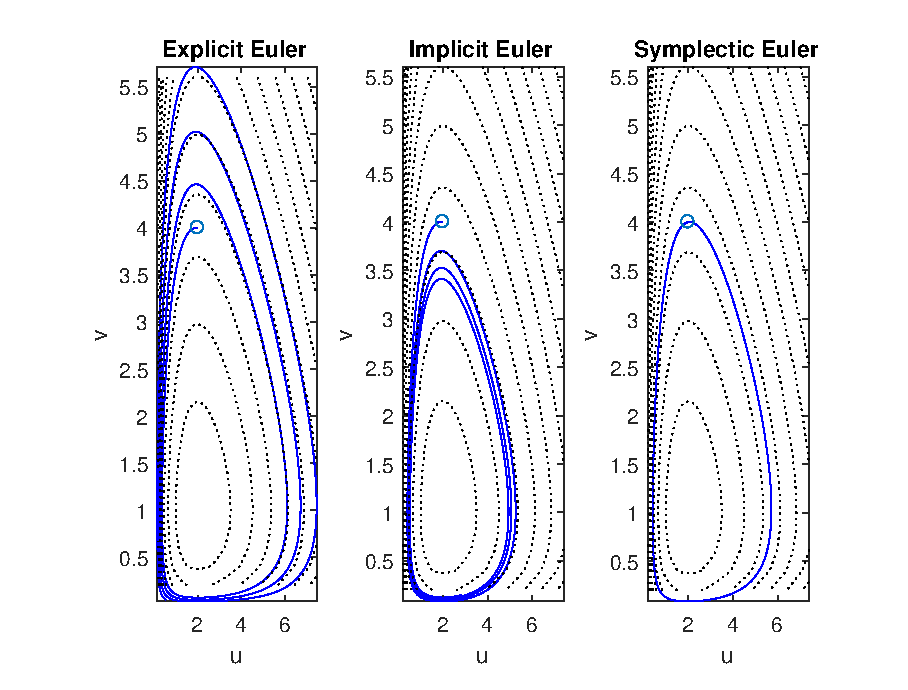
\includegraphics[scale=0.80]{lotka-volterra_method_comparison}
\centering
\caption{Solutions to the Lotka-Volterra Equation}
\label{fig:lotka-volterra_solutions}
\end{figure}

The phase planes in Figure~\ref{fig:lotka-volterra_solutions} convey that the solutions must be a closed loops and periodic - but only the solution using the Symplectic Euler scheme satisifies this criterion. The other two methods qualitatively incorrectly - the solution either spirals inwards or outwards.

Hence, it is important to study methods that preserve qualitative attributes of a system as weell. Since these attributes often occur in differential geometry (the study of differential equations in geometry), we call them geometric invariants - thus lending the name 'Geometric Numerical Integration' to their study.

In this paper, we will focus on a specific class of geometric invariants - non linear, highly oscillatory Hamiltonian problems. We will devote our attention to the problem of molecular dynamics - specifically a simulation of argon molecules as did by A. Rahman \cite{Rahman1964}, and L. Verlet \cite{Verlet1967}. We will first investigate the preservation of geometric invariants in the aforementioned system by the industry standard, Velocity Verlet algorithm, followed by an investigation using the Newmark-Beta family of numerical methods (of which the Velocity Verlet algorithm is a special case).We will conclude with a section on improving the speed of the molecular dynamics simulation, and the effects of improving speed on the action of the above methods.

\end{document}